\chapter{Proposed model of the phenomenon} \label{ch:model}

\section{The model's purpose and description}
Our goal is to build a mobile application that would allow users to review their past walking paths and the current position of their friends. The majority of the effort is focused on implementing a backend API that would filter out corrupted samples and create paths representing routes walked by the user in the past. Frontend mobile application retrieves data from the API and displays it on the map. It also handles all the user interactions and sends current user location.

\section{Algorithm assumptions}
Our algorithm assumes that:
\begin{enumerate}
    \item mobile application is turned on forever,
    \item mobile phones send requests with their location every 5 seconds,
    \item user tracks only outdoor activities,
    \item user cannot walk faster than 14 km/h.
    \item movement with average speed higher than 14 km/h is considered as travel with a vehicle.
\end{enumerate}

Due to the fact that we have limited deployment possibilities, we launched our app with Expo and it is only able to retrieve GPS location when the app is turned on.

\section{Activity cycle diagrams}

\subsection{Front-end app cycle}
The \ref{fig:front} shows the front-end app cycle diagram. The app is very simple in its flow. It simply gets the GPS signal and sends it to the API every 5 seconds. The app also has two modes. One of them allows to see current position of all the users. The second mode displays a history of a specific user.

\begin{figure}[p]
    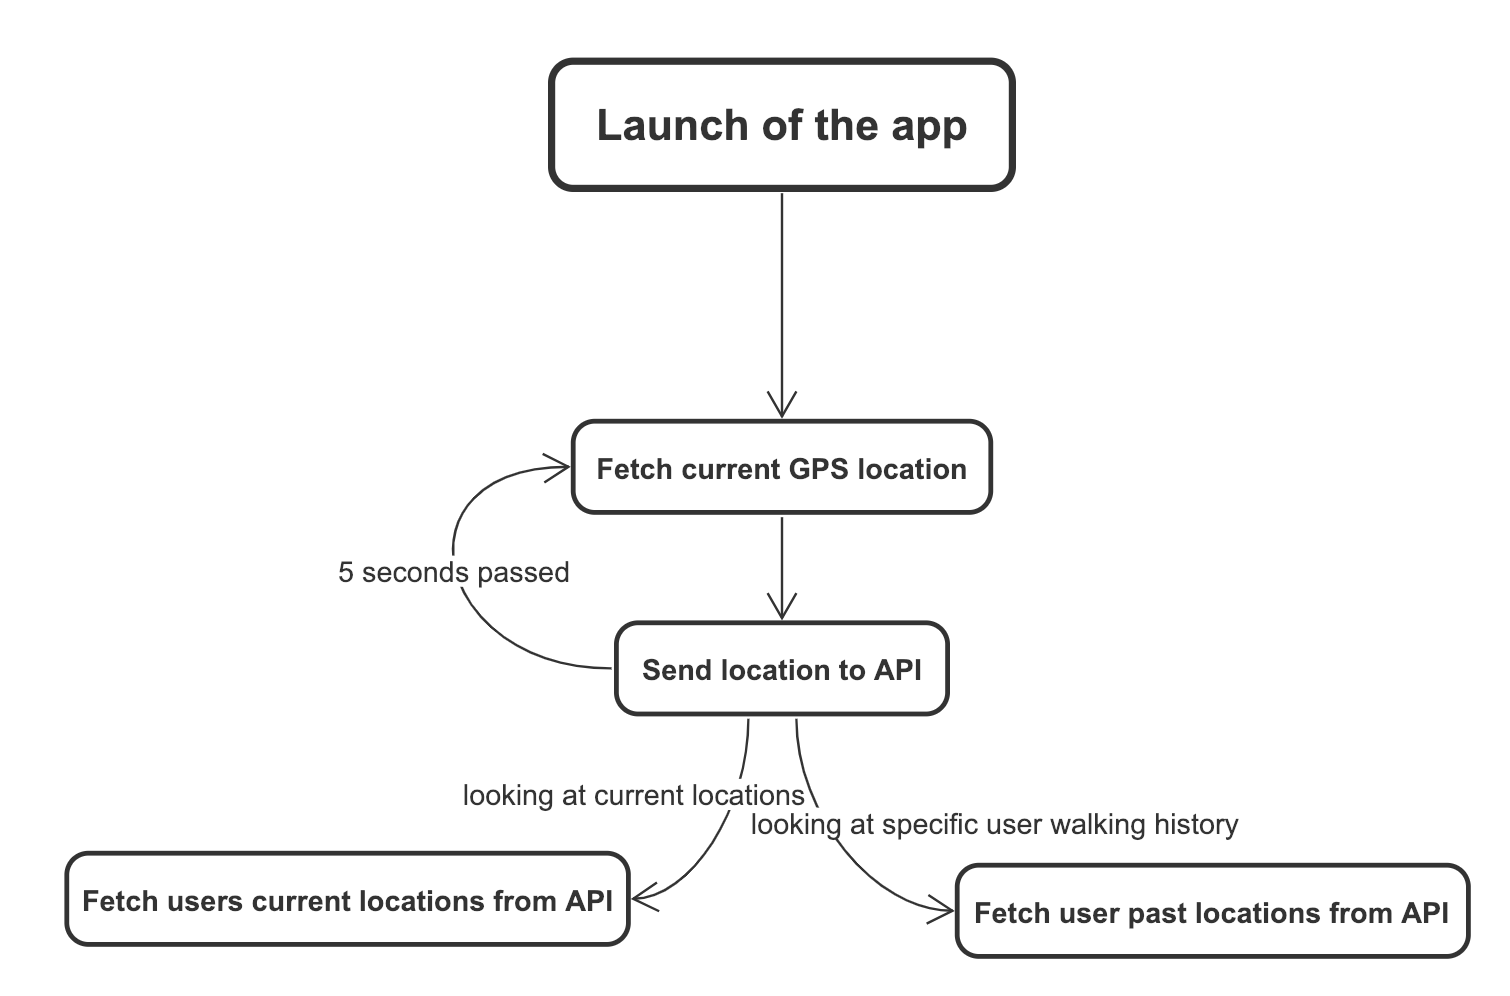
\includegraphics[width=0.9\textwidth]{images/front.png}
    \caption{Front-end app cycle \\ \textit{source: own elaboration}}
    \label{fig:front}
\end{figure}

\subsection{Sending current location to the API}
When the app sends the location along with user's id to the API, the API has to do some calculations depicted in \ref{fig:api} to validate provided data.

\begin{figure}[H]
    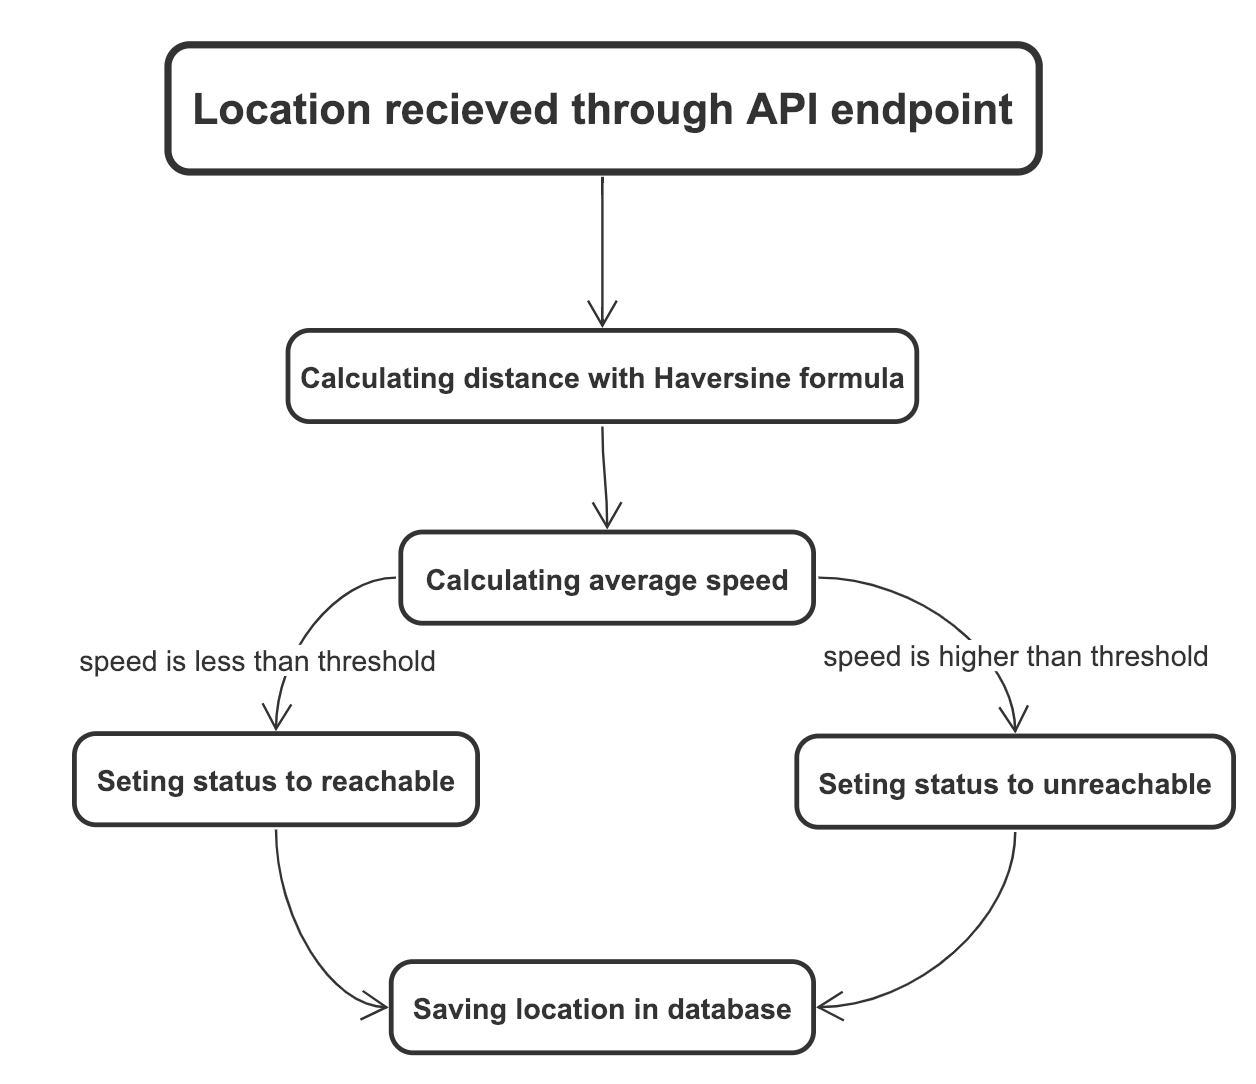
\includegraphics[width=0.9\textwidth]{images/api.png}
    \caption{Sending current location to the API \\ \textit{source: own elaboration}}
    \label{fig:api}
\end{figure}

\subsection{Fetching historical locations}
When the app asks for historical locations, the API calculates on-the-fly if points are reachable and removes all invalid data. This is done every time the app asks for locations to allow tweaking of the algorithm at any moment. If these calculations became expensive, everything could be cached and the cache would be invalidated whenever a new version of the algorithm arrives. The flow can be seen in \ref{fig:history}.

\begin{figure}[p]
    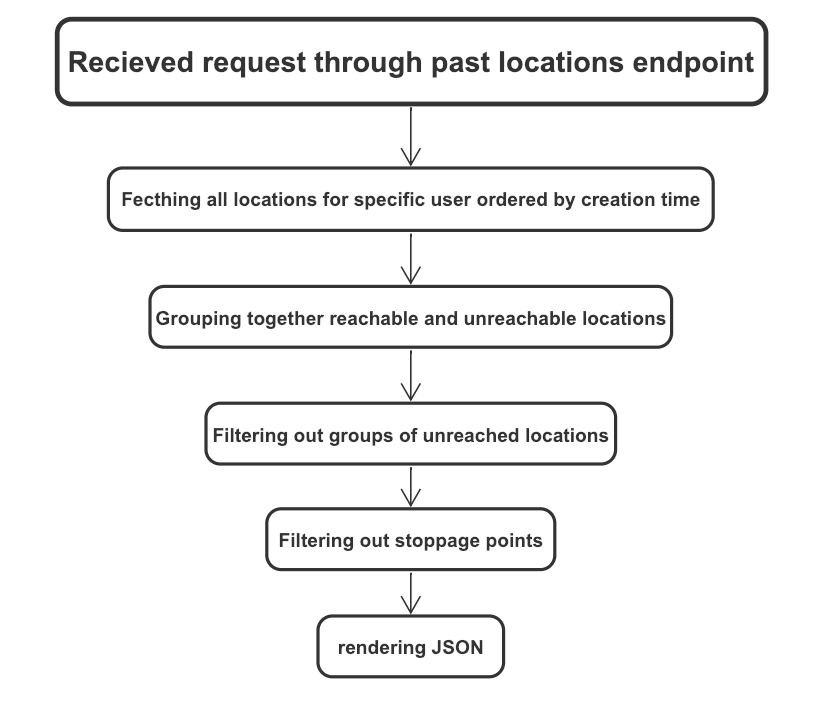
\includegraphics[width=0.9\textwidth]{images/history.png}
    \caption{Fetching historical locations \\ \textit{source: own elaboration}}
    \label{fig:history}
\end{figure}

\section{Applied approach compared to other implementations}

As well as many other engineers we collected locations using GPS technology. In our approach, we used three key components to reach our goal. First of them is calculating the average speed of the user based on his last location and current position. To achieve that we used Haversine formula which is quite unique considering other implementations. Then we experimentally stated some threshold values which were taking into consideration GPS errors. Based on the final judgment we set the status of the location either as reachable or unreachable.

The second one is an algorithm that filters out unreachable locations. In other words, it filters out travelling modes other than walking. This idea is widely known and we thought that it fits our needs.

The third one is a piece of code which aims to remove stoppage points, mainly occurred by traffic light stops and staying in traffic jams. It is our own idea and differs from other projects.

\section{The use case diagram}

\begin{figure}[H]
    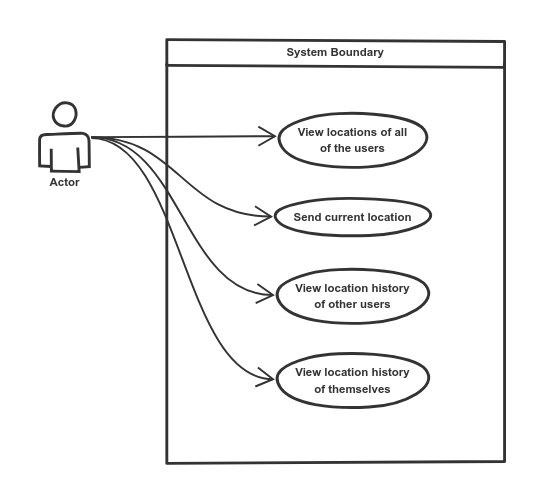
\includegraphics[width=0.9\textwidth]{images/diagram.png}
    \caption{The use case diagram \\ \textit{source: own elaboration}}
\end{figure}
